Una vez descrita la propuesta técnica y visualmente se procede a detallar los distintos pasos seguidos para llevar a cabo la implementación del servicio.\\

\subsection{Conjunto de entrenamiento}
El conjunto de entrenamiento o \textit{dataset} es la información que se utiliza para entrenar a un sistema conversacional en la tarea de reconocer las intenciones expresadas por los usuarios y en responder adecuadamente. Estos datos constan de una serie de definiciones de \textit{intents}, respuestas y patrones de conversación (\textit{stories}) que posteriormente son utilizados por el asistente para tratar identificar correctamente las intenciones expresadas por los usuarios y responder en consecuencia.\\

\subsubsection{\textit{Intents}}
Cada vez que escribimos un mensaje estamos expresando una intención. Los \textit{intents} representan y definen estas intenciones recopilando una gran cantidad de ejemplos reales. Al construir el conjunto de  entrenamiento es importante tener en cuenta que una determinada intención puede ser expresada de distintas maneras. Pongamos por caso la pregunta  \textit{¿Existe cura para el VIH?} extraída de la hoja de cálculo. La cuestión expresa la intención del usuario de querer saber si existe algún tratamiento que cure completamente el VIH. Sin embargo, esta es simplemente una  de las múltiples formas que existen de preguntarlo, pues sería igualmente posible formular \textit{¿Hay cura para el VIH?} o \textit{¿El VIH tiene cura?} expresando la misma intención.\\

Por tanto, un usuario puede expresar la misma intención a través de diferentes expresiones. Por ello, cada pregunta se debe analizar para identificar la intención, y en base a esta, elaborar una serie de variaciones que garanticen un amplio espectro de reconocimiento.
Estas variaciones consisten en:

\begin{itemize}
	\item Reformulaciones parciales o completas de las preguntas.
	\item Variantes con faltas de ortografía.
	\item Variantes con errores de escritura.
\end{itemize}

Por tanto, y siguiendo con el ejemplo anterior, para \textit{¿Existe cura para el VIH?} se pueden obtener las siguientes variaciones:

\begin{verbatim}
- intent: cura_vih
  examples: |
    - ¿Existe cura para el VIH?
    - existe ya cura para el vih?
    - han inventado alguna cura para el vih?
    - que cura hay para el vih?
    - se puede sanar el vih?
    - es posible expulsar el virus del cuerpo?
    - es posible exulsar el vih?
    - tiene cura el sida?
    - como se cura elsida?
    - puede alguienr ecuperarse completamente del vih?
    - ...
\end{verbatim}

Es importante considerar que para posteriormente el modelo generado distinga de forma fiable una intención de otra los ejemplos deben ser distintos entre los \textit{intents}. Es decir, no se debe utilizar el mismo ejemplo de entrenamiento para dos intenciones diferentes. Si los ejemplos de entrenamiento resultan demasiado similares, se produce una confusión de intenciones \cite{bestPracticesNLU}. En esta fase inicial se generan manualmente 30 variaciones por intención para garantizar unos resultados suficientemente satisfactorios para el prototipo [ref rasa]. En las siguientes fases del desarrollo las variaciones aumentarán con la recogida de datos reales (ver sección \ref{cdd}).

\subsubsection{Respuestas}
Las respuestas proporcionadas por el hospital son en muchos casos de difícil asimilación por parte de los usuarios. En su mayoría, utilizan un registro muy formal que dificulta que el usuario establezca un vínculo con el \textit{bot}. Además, en muchos casos la longitud del mensaje es excesivo, lo que puede provocar rechazo y saturación [referencia]. Por lo general, al chatear los usuarios suelen usar mensajes cortos, y en consecuencia, es recomendable sintetizar y aportar sólo la información relevante [referencia].\\

Por tanto, es necesario aplicar distintas técnicas para dinamizar las respuestas y no aborrecer al usuario. La información debe ser concreta, responder directamente a la pregunta y en la medida de lo posible intentar captar su intención. Esta tarea se realiza mediante la introducción de modificaciones tales como:

\begin{itemize}
	\item División de las respuestas más largas en varios mensajes.
	\item Ligeros cambios para variar el registro por otro menos formal.
	\item Supresión de afirmaciones y negaciones rotundas para adaptar las respuestas a una mayor variedad de preguntas.
	\item Hacer uso de algunos emoticonos para amenizar a ciertas expresiones o datos.
\end{itemize}

Dado el carácter informativo del servicio estas alteraciones se introducen intentando encontrar un equilibrio entre la calidad de la información y la síntesis. Como ejemplo, en la figura \ref{fig:modified response} se puede observar la respuesta original a la pregunta \textit{¿Qué es la Infección aguda por el VIH?} y su versión final tras las modificaciones.

\begin{figure}[htbp]
\centering

\includegraphics[scale=0.3]{../images/original_response.png}
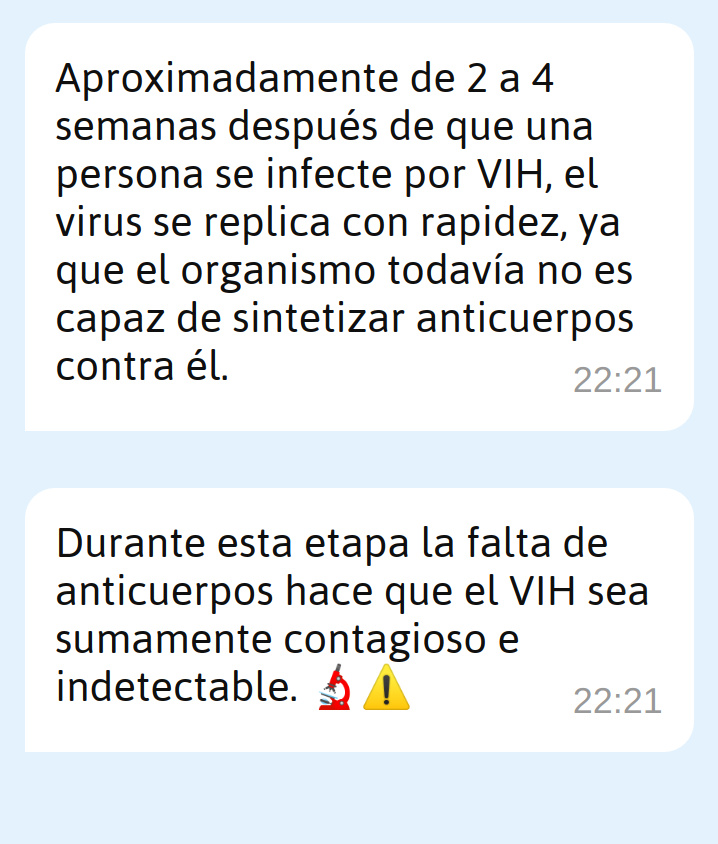
\includegraphics[scale=0.3]{../images/modified_response.png}
\caption{Ejemplo de transformación de una respuesta}
\label{fig:modified response}
\end{figure}

\subsubsection{\textit{Stories}}
Una vez el conjunto de entrenamiento cuenta con la información de los \textit{intents} para identificar las expresiones y sus correspondientes respuestas, es necesario indicarle como debe utilizarlas. Para ello, se incorpora también a los datos de entrenamiento estructuras o patrones de conversación denominadas \textit{stories}. Las historias o \textit{stories} son representaciones de conversaciones entre usuarios y el chatbot. Estos datos utilizan un formato específico en el que la información introducida por el usuario se expresa como \textit{intents} y las respuestas como acciones del asistente \cite{rasaStories}. Por tanto, los \textit{intents} permiten identificar las intenciones, las respuestas contienen la información que recibirá el usuario, y las historias aportan el contexto y la lógica necesaria para responder coherentemente.\\

\begin{verbatim}
  - story: Pregunta por la cura + casos que se han curado + paciente berlin
    steps:
      - intent: cura_vih
      - action: utter_cura_vih
      - intent: faq/casos_cura
      - action: utter_faq
      - intent: faq/paciente_berlin
      - action: utter_faq

  - story: Agradecer + necesita algo más
    steps:
      - intent: agradecer
      - action: utter_no_hay_de_que
      - action: utter_algo_mas
      - intent: afirmar
      - action: utter_ofrecer_ayuda
\end{verbatim}

Tras procesar toda esta información y realizar el entrenamiento \textit{Rasa} genera un modelo con el cual el asistente es capaz de analizar las preguntas realizadas por los usuarios, asociarlas a uno de los \textit{intents} que ya tenga definidos (en base a una probabilidad) y ofrecer la respuesta correspondiente según le haya sido indicado.\\

Con la intención de que el chatbot pueda mantener conversaciones lo más completas posibles se han añadido al conjunto de entrenamiento \textit{intents}, respuestas y historias pertenecientes a 3 áreas distintas: conocimiento médico, expresiones auxiliares y cháchara. Los datos médicos están orientados ha responder todas las dudas médicas sobre el VIH y han sido extraídos de la hoja de cálculo facilitada por parte de la Unidad de Enfermedades Infecciosas del Hospital General de Elche. Este documento consta de 130 preguntas con sus correspondientes respuestas y contiene todo el conocimiento médico que inicialmente tendrá el chatbot.\\

A parte de todas las cuestiones relacionadas con el VIH el asistente debe ser también capaz de entender y desenvolverse con una serie de expresiones básicas que suelen formar parte un diálogo. Las conversaciones suelen empezar con un \textit{Hola} o \textit{¡Buenos días!} y suelen ser correspondidas con otro saludo, seguidas de un \textit{¿Cómo estás?} o \textit{¿Cómo va?} y sus correspondientes respuestas. Durante el transcurso, también pueden aparecer otras expresiones como afirmaciones o negaciones (\textit{¡Por supuesto!}, \textit{Claro}, \textit{Para nada} etc) o peticiones como \textit{¿Me puedes ayudar?} o \textit{Necesito tu ayuda}. Finalmente, se suele usar un \textit{Adiós} o \textit{Hasta luego} para despedirse y finalizar la conversación.\\


Todas estas expresiones y mucha otras aparecen tarde o temprano en cualquier conversación, y por tanto, se ha incorporado el mayor numero posible de ellas al conjunto de entrenamiento.\\


\begin{figure}[htbp]
\centering

\includegraphics[scale=0.15]{../images/basics_chat.png}

\includegraphics[scale=0.15]{../images/basics_chat_2.png}
\caption{Ejemplo de una pequeña conversación}
\label{fig:expresiones auxiliares}
\end{figure}


Durante el devenir de una conversación es bastante probable que el usuario le realice una pregunta al chatbot que esté fuera de su ámbito de conocimiento, y que por tanto, no sepa responderla. A este suceso se le llama desvíarese de happy path. Dentro de lo posible hay que intentar controlar estos desvíos y preparar al asistente para que pueda responder a los más comunes. Algunos de los ejemplos más repetidos son \textit{¿Cómo te llamas?}, \textit{¿Eres un robot?}, \textit{Que tiempo hace} [ref paper].

[imagen ejemplo  chitchat]


\subsubsection{Manejo de mensajes fuera de ámbito}
Por otra parte, alredeor de un 12 por cien de las personas que  [referencia paper] los chatbots suelen ser objeto de insultos.
[imagen ejemplo out of scope ingles,insulto]

\cite{bestPracticesNLU}

\subsubsection{Manejo de errores}
Por último, hay que asumir que tarde o temprano, por muy bien diseñado que esté un chatbot habrá un momento donde no sepa identificar correctamente una pregunta y falle.

Por otra parte, también debe estar preparado para no te he entendido, no sabes hacerlo etc

[imagen ejemplo recuperación ante fallo, pregunta si puede repetir]

\subsection{Servidor}

\subsection{Aplicación web}
Desarrollo del frontend

\subsection{Despliegue}
Una vez implementados el servidor y el \textit{frontend} web es necesario publicar una versión de prueba del servicio para poder empezar con la fase de obtención de datos de conversaciones reales. Para ello, la Universitat Politècnica de València pone a disposición del proyecto una maquina virtual con \textit{Ubuntu 18.04} donde poder realizar el despliegue. Mediante acceso \textit{SSH} se instalan todas las librerías necesarias (\textit{apache}, \textit{python}, \textit{rasa}, \textit{spacy} etc) y se ponen en marcha tanto la web como el servidor conversacional.\\

Una vez el sistema está funcionando se realiza una pequeña prueba para asegurarse que la recogida de datos funciona correctamente. Tras un resultado satisfactorio se solicita a la universidad la apertura de los puertos 80, 5055 y 5005 para que los usuarios externos puedan acceder y probar el chatbot.\\


\subsection{Desarrollo basado en conversaciones}
\label{cdd}
Uno de los mayores poblemas que se suelen presentar durante el desarrollo de un chatbot es que inicialmente, el dataset suele estar creado por les dasaroladores, muy sesgado y alejado de siatuaciones reales. El desarrollo basado en conversaciones (\textit{Conversation-Driven Development}) es el proceso de escuchar a los usuarios y utilizar esa información para mejorar el asistente \cite{conversationDriven}. Programar chatbots robustos puede ser un auténtico reto pues los usuarios siempre dirán algo que inicialmente no estaba contemplado en el conjunto de entrenamiento. En consecuencia, este enfoque es la mejor manera de solucionar esta problemática, pues toda nueva información se incorpora al \textit{dataset} y así el modelo se nutre de situaciones y expresiones reales. Esta estrategia está especialmente recomendada por los desarrolladores de \textit{Rasa} \cite{bestPracticesNLU}.\\

Tras publicar la primera versión de prueba del chatbot el proyecto se encuentra listo para entrar en esta fase de desarrollo centrada en la recogida de datos. Para ello, durante varias semanas se compartirá el chatbot, se revisarán las conversaciones obtenidas, y se anotarán, clasificarán e incorporarán al \textit{dataset} todos los datos recopilados. Tras realizar todos estos cambios sobre el conjunto de entrenamiento se ejecutarán los \textit{tests} correspondientes, se corregirán posibles errores y se volverá a compartir el chatbot para una nueva iteración.\\

\begin{figure}[htbp]
\centering
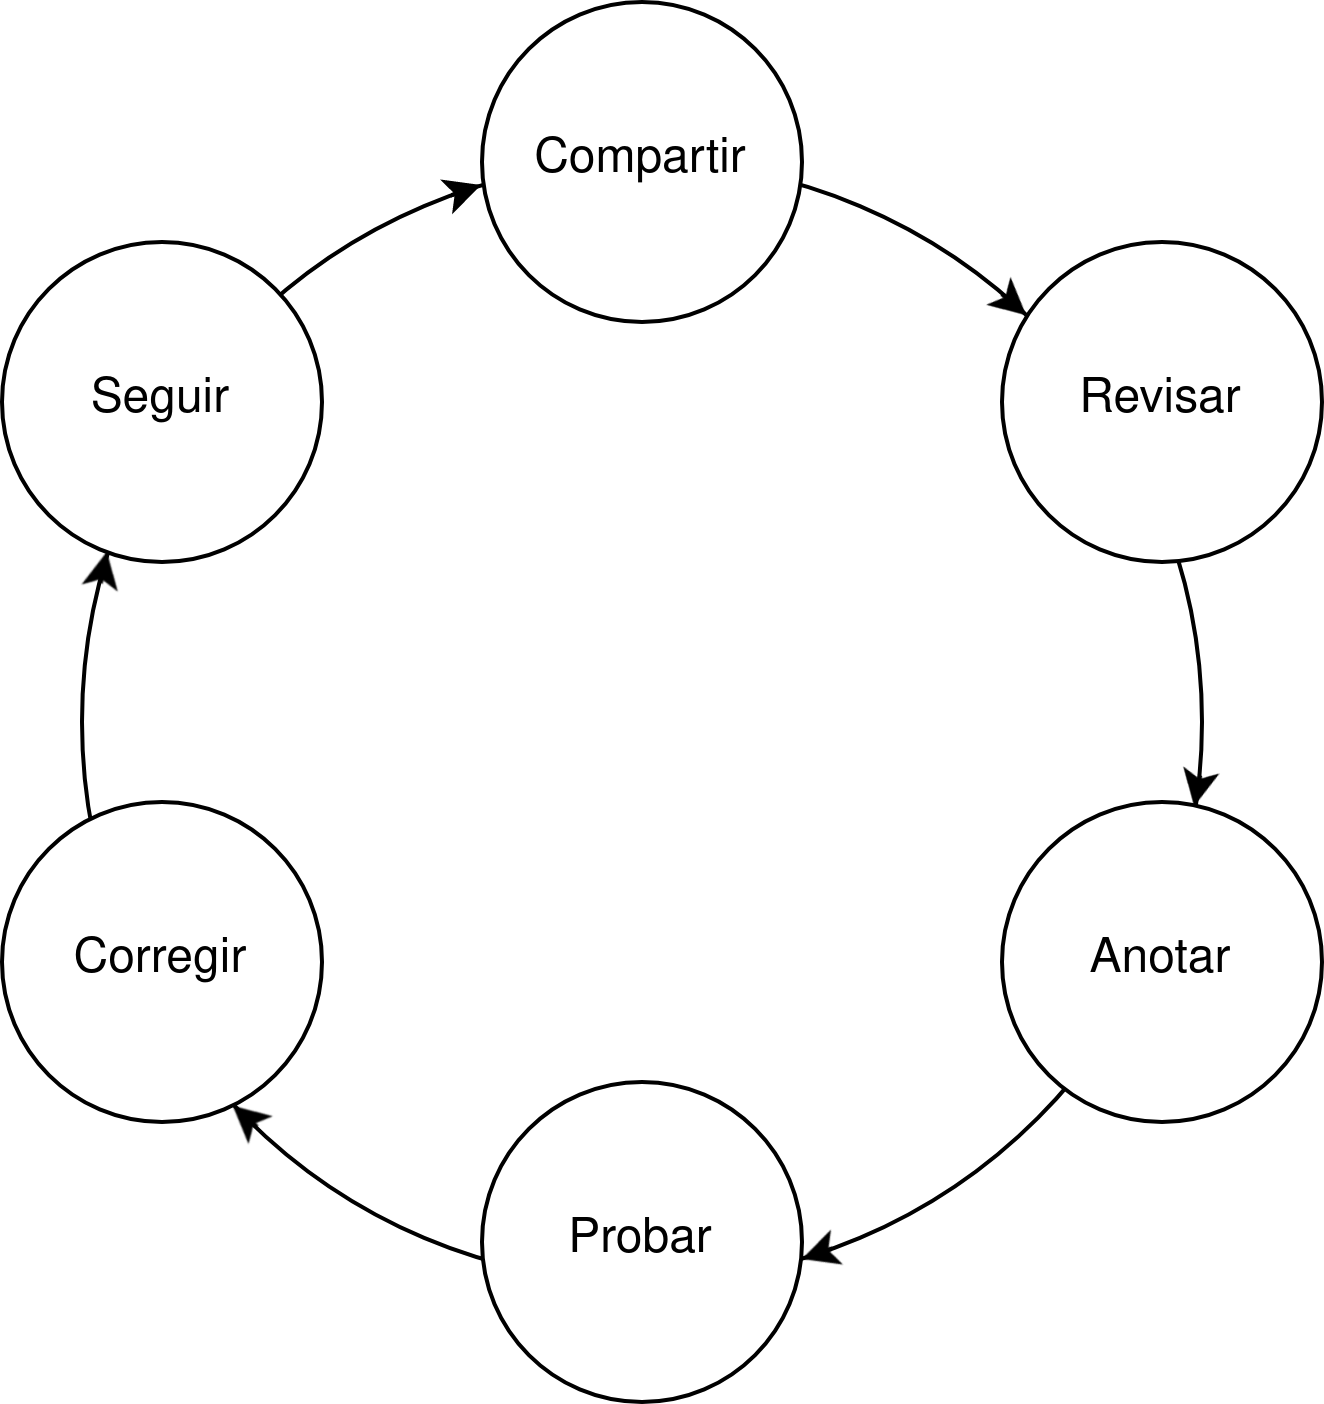
\includegraphics[scale=0.15]{../images/cdd.png} 
\caption{Ciclo del desarrollo basado en conversaciones}
\label{fig:cdd}
\end{figure}

Se trata de etiquetar, clasidficar, encontrar fallos, flowas ...\\	

\begin{figure}[htbp]
\centering
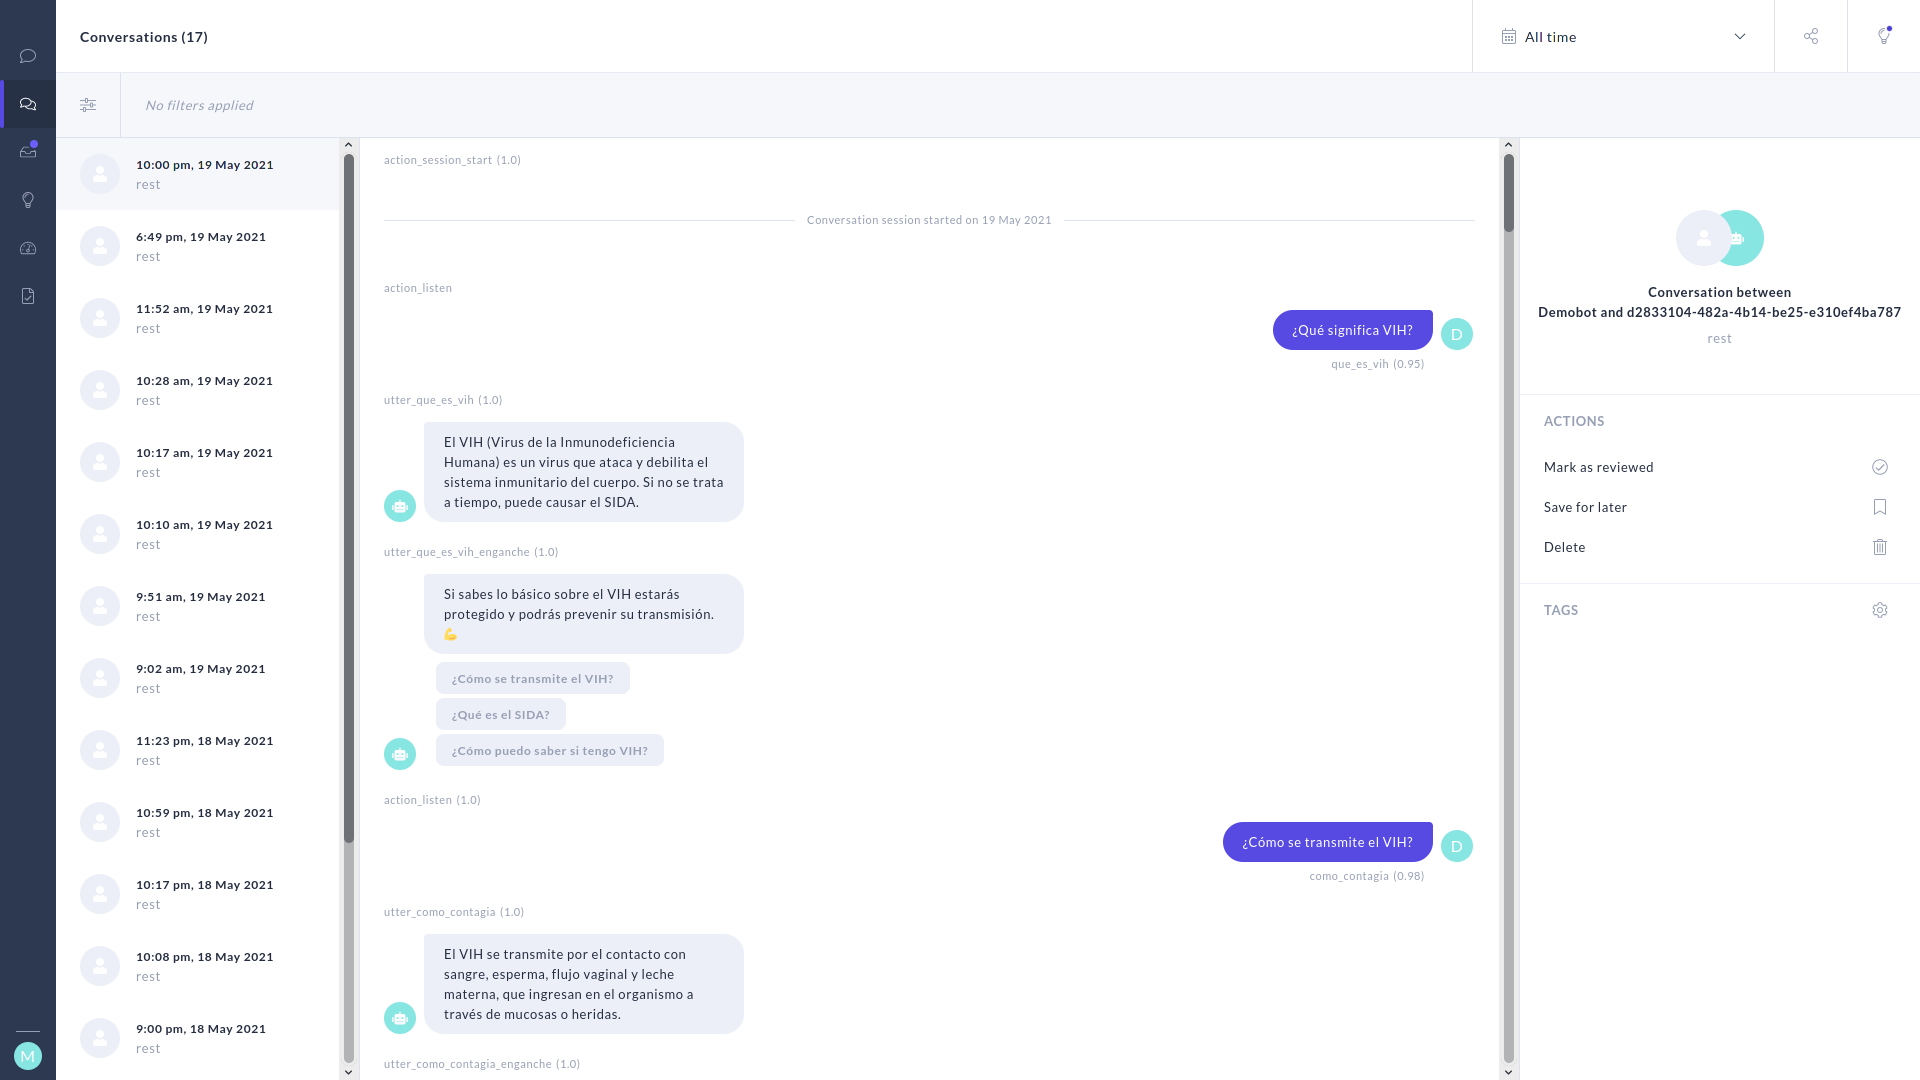
\includegraphics[scale=0.3]{../images/collected_dialogs.png} 
\caption{Ejemplo de una de las conversaciones recogidas}
\label{fig:collected dialogs}
\end{figure}

Durante todo este proceso se recogieron y analizaron aproximadamente 23 conversaciones de las cuáles se pudo extraer e incorporar a la base de conocimiento la siguiente información:\\

\begin{itemize}
	\item 30 preguntas nuevas que inicialmente no estaban previstas.
	\item 204 datos NLU
\end{itemize}


\begin{figure}[htbp]
\centering
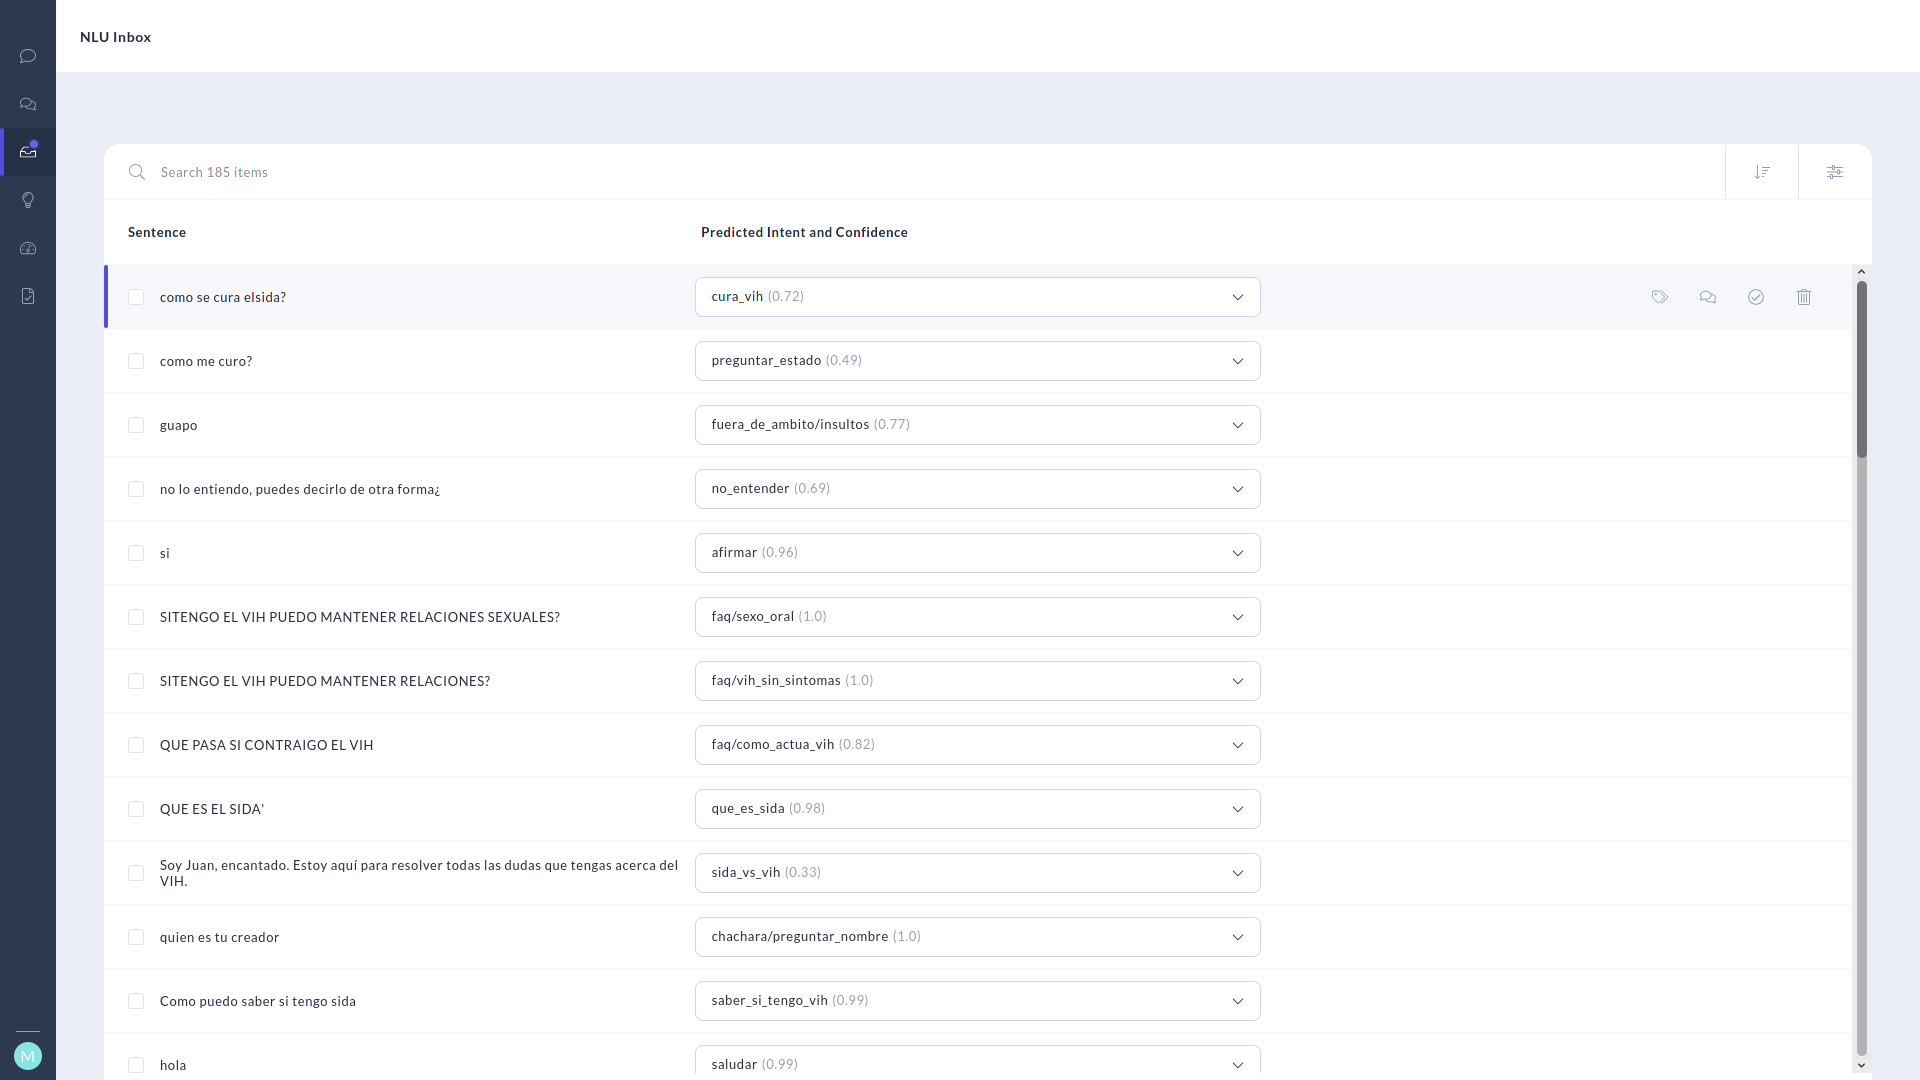
\includegraphics[scale=0.3]{../images/collected_nlu.png} 
\caption{Datos NLU recopilados y su etiquetado}
\label{fig:collected nlu}
\end{figure}


\subsection{Distribución}
Teniendo en cuenta el carácter del servicio se propone que el chatbot se ponga a disposición del público a través de una web de libre acceso y sin requerir registro. El objetivo es facilitar a los usuarios el acceso para que cualquier persona pueda acceder al servicio sin necesidad de introducir ningún dato personal ni instalar ninguna aplicación en su terminal. \\

Para aquellos usuarios que lo deseen se empaquetará la web en una aplicación tanto para \textit{Android} como para \textit{iOS} utilizando el framework \textit{Capacitor}. Esto permite que aquellos usuarios interesados puedan instalar el servicio desde las tiendas de aplicaciones habituales en sus dispositivos móviles.\\


[TODO: Recogida de conversaciones reales y etiquetado]



